\documentclass[a4paper,norsk]{article}
\usepackage[utf8]{inputenc}
\usepackage[T1]{fontenc,url}
\usepackage{babel,textcomp}
\usepackage{graphicx}
\usepackage{amsmath}
\usepackage{cleveref}
\usepackage[cmyk]{xcolor}
\usepackage{listings}

\lstset {language=C++,    
backgroundcolor=\color{yellow!20},    
commentstyle=\color{green},    
%keywordstyle=\color{blue},    
basicstyle=\footnotesize}
\urlstyle{sf}
\title{Oblig 1 ADS101}
\date{\today}
\author{Adam Aske}
\newpage
\begin{document}
\maketitle
\tableofcontents
\newpage

\section{Introduksjon}
Her bruker jeg algoritmen Selection Sort og C++ sin innnebygde funskjon Sort til å sortere arrayer av forskjellige størrelser. 
Chrono tar tiden på hvor lang tid det tar for arrayer av forskjellige størrelser. 
Målingene er gjennomsnittet av algorytmene som har blitt kjørt 10 ganger per N.

\section{Selection Sort}Selection sort algoritmen på int arrayer av forskjellige størrelser.
Funkjsonen tar inn en array og en størrelse. Først blir arrayen fylt med tilfeldige tall. 
\begin{lstlisting}[language=C++, caption={main.cpp}]
template<typename T, size_t N>
void SelectionSort(T (&arr)[N], std::ofstream &file){

    for (int i = 0; i < N; i++){
        arr[i] = rand();
    }

    auto start = std::chrono::high_resolution_clock::now();
    //1. Selection sort
    for(auto i = 0; i < N-1; i++){
        for(auto j = i +1; j < N; j++){
            if(arr[j] > arr[i]){
                std::swap(arr[j], arr[i]);
            }
        }
    }

    //Get the end
    auto end = std::chrono::high_resolution_clock::now();
    std::chrono::duration<double> totalTime = end-start;
    std::chrono::nanoseconds totalTimeNano = 
    	std::chrono::duration_cast
    		<std::chrono::nanoseconds>(totalTime);
    totalTime += totalTimeNano;
    int time = std::chrono::duration_cast<std::chrono
		::nanoseconds>(end-start).count();
    std::cout << "With " << N << " elements, it took " 
		<< totalTime.count() 
    << " nanoseconds to sort
	 them doing the selection sort alagorithm."
	 << std::endl;
    file << totalTime.count() << std::endl;
    selectionTimes.push_back(totalTime.count());
}
\end{lstlisting}
\subsection{Selection Sort Results}
\begin{figure}
\centering
	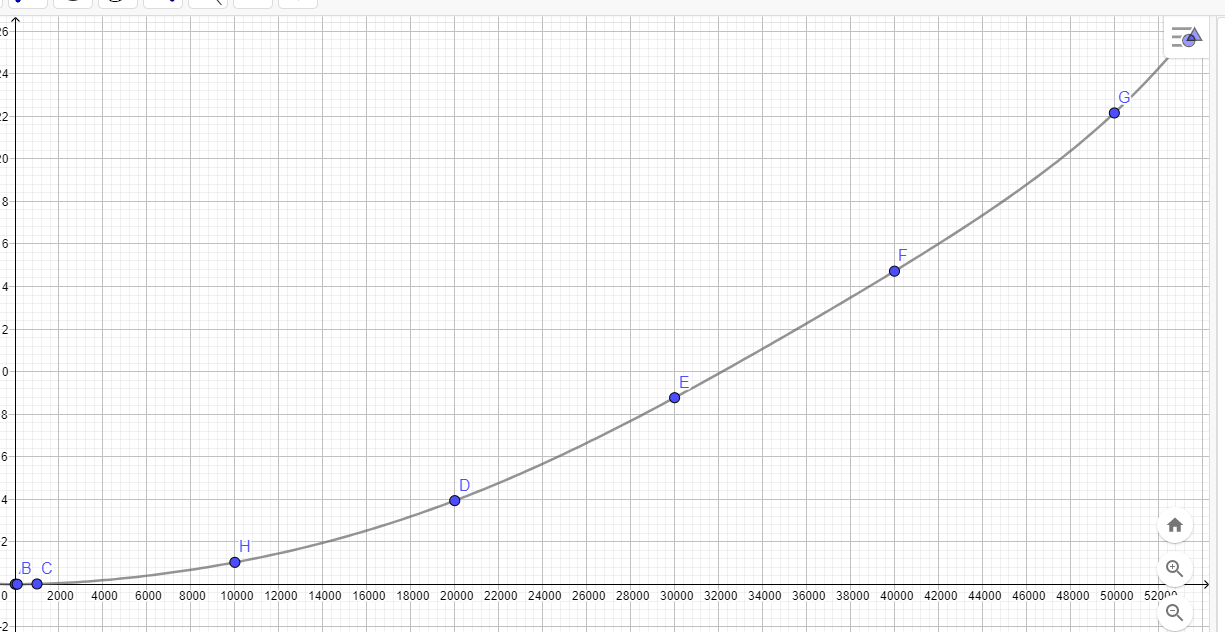
\includegraphics[width =3in]{SelectionSortGraph.png}
	\caption{X-Aksen er antall elementer i arrayet og Y-Aksen er tiden det tokk for å sortere elementene etter størrelse}
\end{figure}
\newpage
\section{Std::Sort}Std::Sort funkjsonen brukes på de samme arrayene. Funkjsonen tar inn en array og en størrelse. Først blir arrayen fylt med tilfeldige tall. 
\begin{lstlisting}[language=C++, caption={main.cpp}]
template<typename T, size_t N>
void StdSort(T (&arr)[N], std::ofstream &file){
    //2. Std::sort
    auto start = std::chrono::high_resolution_clock::now();

    std::sort(std::begin(arr), std::end(arr));

    auto end = std::chrono::high_resolution_clock::now();

    std::chrono::duration<double> totalTime = end-start;
    std::chrono::nanoseconds totalTimeNano = 
	std::chrono::duration_cast
<std::chrono::nanoseconds>(totalTime);
    totalTime += totalTimeNano;
    int time = std::chrono::duration_cast
	<std::chrono::nanoseconds>(end-start).count();
    std::cout << "With " << N << 
	" elements, it took " << totalTime.count() 
	<< " nanoseconds to sort them using std::sort." 
<< std::endl;
    file << totalTime.count() << std::endl;
    stdSortTimes.push_back(totalTime.count());
}
\end{lstlisting}



\section{Std::Sort Resultat} 
Resultat
\begin{figure}
	\centering
	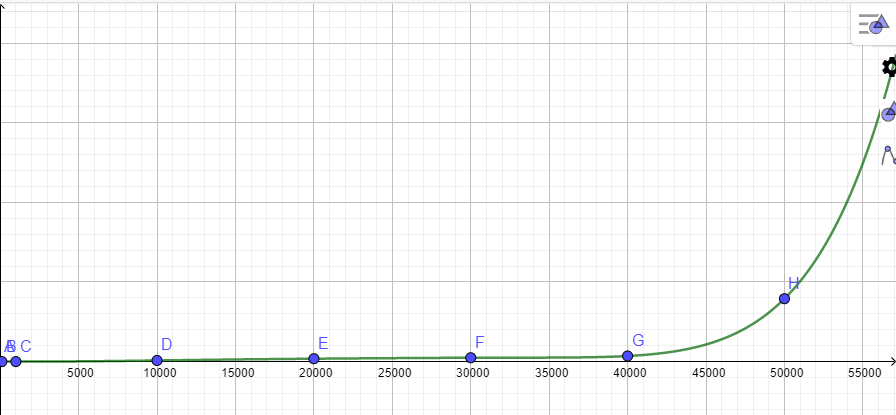
\includegraphics[width =3in]{StdSortGraph.png}
	\caption{X-Aksen er antall elementer i arrayet og Y-Aksen er tiden det tokk for å sortere elementene etter størrelse}
\end{figure}
\end{document}